\section*{Das Perzeptron}

Der Aufbau eines typischen Perzeptrons besteht aus einer oder mehreren Schichten sogenannter \textit{Linear Threshold Units} (LTU) wie in Abbildung \ref{ltu} dargestellt.

\begin{figure}[H]
	\begin{center}
		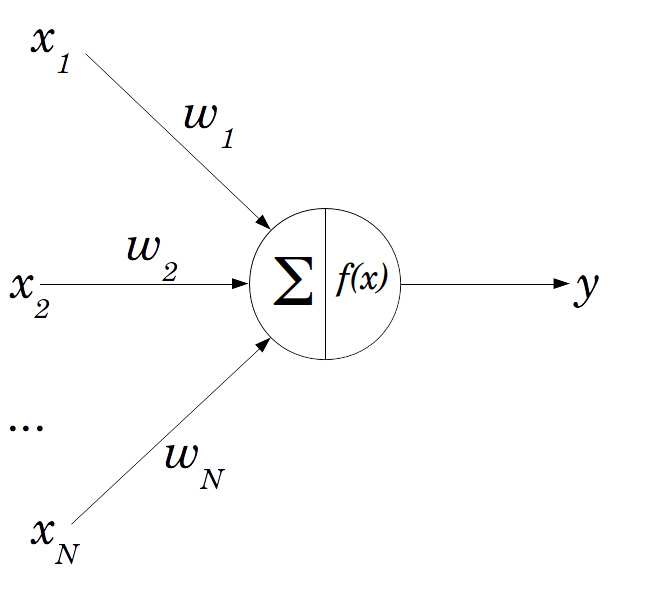
\includegraphics[width=7cm]{Bilder/perceptron.png} 
		\caption[Linear Threshold Unit]{Linear Threshold Unit \cite{AurelienGeron.2018}}
		\label{ltu}
	\end{center}
\end{figure}

Es besteht aus $n$ Eingängen mit $x_{i} \in \mathbb{Q}$, die im Inputvektor $\boldsymbol{x}$ zusammengefasst werden. Jeder Eingang wird mit einem Gewicht $w_{i}$ aus dem Gewichtsvektor $\boldsymbol{w}$ versehen. Die LTU berechnet das Skalarprodukt $\boldsymbol{w}^{T} \circ \boldsymbol{x}$ aller Eingänge $\boldsymbol{x}$ mit ihren Gewichten $\boldsymbol{w}$ und wendet anschließend auf das Ergebnis $z$ eine Aktivierungsfunktion an. Das Ergebnis $h_{w}(x)$ kann anschließend als Eingabe für ein weiteres Perzeptron dienen.

Die einfachste Aktivierungsfunkion für ANNs ist die \textit{Heaviside-Funktion} \cite{AurelienGeron.2018}: 

\begin{equation} \label{heaviside}
\begin{split}
h_{w}(x) = s(\boldsymbol{w}^{T} \circ \boldsymbol{x}) = s(z) = \\\ \begin{pmatrix} 
w_{1}&&w_{2}&&\dots&& w_{n}\\ 
\end{pmatrix} 
\circ 
\begin{pmatrix} x_{1}\\
x_{2}\\
\vdots\\
x_{n}\\
\end{pmatrix}) = 
\begin{cases}
1 & \text{wenn} z \geq 0 \\
0 & \text{wenn} z < 0 .\\
\end{cases}
\end{split}
\end{equation}
\equations{Die Heaviside-Funktion}

Falls eine Klassifizierung mit Wahrscheinlichkeiten vorliegen soll, so ist die letzte Schicht eines Perzeptrons meist mit der \textit{Softmax-Funktion}

\begin{center}
$
h_{w}(x) = \sigma(z)_j = \frac{e^{z_j}}{\sum_{i=0}^n e^{z_i} }
$
\end{center}

implementiert, die den Wert des $j$-ten LTUs einer Schicht mit allen anderen $n$ Werten der LTUs derselben Schicht ins Verhältnis setzt \cite{AurelienGeron.2018}. Es gibt eine Vielzahl an möglichen Aktivierungsfunktionen, die im Kapitel \textit{Hyperparameter} betrachtet werden.

Die Aktivierung einer LTU hängt zusätzlich von einem Schwellwert $\theta$ ab, der durch einen sogenannten \textit{Bias} festgelegt wird. Dies ist die Gewichtung des letzten Eingangs, der standardmäßig den Wert 1 liefert. Wird die Gewichtung negativ gewählt, so ist es schwieriger die LTU zu aktivieren, während eine positive Gewichtung die Aktivierung vereinfacht \cite{AurelienGeron.2018}.

Nun bilden ein oder mehrere Schichten solcher LTUs ein Perzeptron. Jede einzelne LTU ist dabei mit allen LTUs der vorherigen Schicht verbunden (siehe Abbildung \ref{neural_network}). Hier wird auch von sogenannten vollständig verbundenen Schichten (engl.: \textit{Fully-Connected Layer}) gesprochen. Die beiden LTUs zur Ausgabe können dabei Aussagen über eine Klassifikation von Daten anhand der Eingangsdaten treffen, während die LTUs im Input Layer wesentlich Daten weiter reichen. Die Verbindungen zur ersten Schicht des Hidden Layer sind stets mit Eins belegt. Existiert keine verborgene Schicht, so wird das ANN als einschichtiges Perzeptron bezeichnet, ab einer oder mehr verborgenen Schichten wird bereits von einem \textit{Multi-Layer Perzeptron} (MLP), einem mehrschichtigen Perzeptron, gesprochen. Ist das neuronale Netz optimal trainiert, so ist am Ende nur eines der LTUs zur Ausgabe aktiviert. Das folgende ANN ist zudem ein Beispiel für ein sogenanntes \textit{Feed-Forward Network}, bei dem die Auswertung der Daten von einer Schicht zur nächsten weitergereicht wird, ohne zu bereits besuchten Schichten zurückzukehren \cite{AurelienGeron.2018}.

\begin{figure}[H]
	\begin{center}
		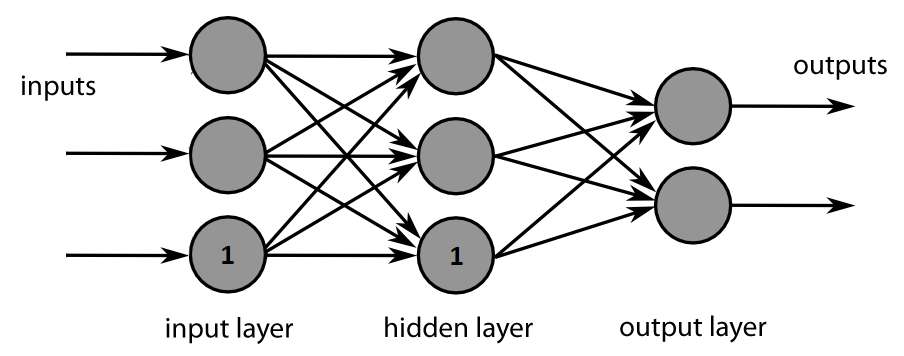
\includegraphics[width=12cm]{Bilder/neural_network.png} 
		\caption[Das einschichtige Perzeptron]{Das einschichtige Perzeptron \cite{Wikipedia.20190123}}
		\label{neural_network}
	\end{center}
\end{figure}

\section*{Lernmethoden}

Im Wesentlichen existieren vier Methoden, mit deren Hilfe neuronale Netze trainiert werden können. Beim \textit{überwachten Lernen} werden den Trainingsdaten Lösungen, sogenannte \textit{Labels}, hinzugefügt. Klassifikationsprobleme stellen eine typische Problemstellung für überwachte Lernverfahren dar. Auch die später eingeführten Objektdetektoren werden mittels überwachtem Lernen trainiert \cite{AurelienGeron.2018}. 

Beim \textit{unüberwachten Lernen} werden den Trainingsdaten keinerlei Lösungen hinzugefügt, der Algorithmus muss selbstständig Klassifikationsaussagen treffen können. Ein Beispiel hierzu wäre \textit{K-Means Clustering} \cite{AurelienGeron.2018}. 

\textit{Deep Belief Networks} (DBNs) bestehend aus einzelnen \textit{Restricted Boltzmann Machines} (RBMs) werden zunächst unüberwacht trainiert, bevor im \textit{Fine Tuning} das Gesamtnetzwerk mit überwachten Lerntechniken fertiggestellt wird. Es wird hier von \textit{halbüberwachtem Lernen} gesprochen.

Als letztes ist das sogenannte \textit{Reinforcement Learning} zu nennen. Hierbei wird ein neuronales Netz durch das Erteilen von Belohnungen bzw. Bestrafungen so konditioniert, dass es zukünftig basierend auf der wahrgenommenen Umwelt selbstsicher richtige Aktionen auswählen kann.

\section*{Gradientenverfahren und Backpropagation}

Um zu verstehen, wie ein neuronales Netz durch überwachtes Lernen \glqq lernt\grqq{}, muss zunächst der Begriff der Kostenfunktion (engl.: \textit{cost function}) eingeführt werden. Die Kostenfunktion ist ein Qualitätsmaß dafür, wie weit die Ausgabe einer LTU vom erwarteten Wert abweicht \cite{AurelienGeron.2018}. Angenommen dem neuronalen Netz wird ein Datensatz zur Klassifikation übergeben, so ist am Ende meist nicht nur eine LTU zu Ausgabe aktiviert, was auf eine eindeutige Klassifikation schließen würde, sondern meist mehrere zu einem frühen Stadium des neuronalen Netzes.

Eine oft genutzte Kostenfunktion ist die \textit{Root Mean Squared Error Funktion} (RMSE):

\begin{equation} \label{mse}
E(\boldsymbol{z},\boldsymbol{o}) = \sqrt{\frac{1}{n}\sum_{k=0}^n (z_k-o_k)^2}.
\end{equation}
\equations{Die RMSE-Funktion}

Eine weitere Kostenfunktion für das überwachte Lernen ist die \textit{Smooth L1} Funktion:

\begin{center}
$
SM_{L1}(\boldsymbol{z},\boldsymbol{o}) = \begin{cases}
\sum_{k=0}^n 0.5(z_k-o_k)^2      & \text{wenn } |x| < 1\\
\sum_{k=0}^n |z_k-o_k| - 0.5   & \text{sonst}
\end{cases}
$
\end{center}

Bei beiden ist $z$ der erwartete Ausgabevektor des Perzeptrons, während $o$ die momentane Ausgabe darstellt. Den Fehler der Abweichung dieser beiden Werte gilt es nun schrittweise zu minimieren. Um dies zu erreichen können die drei Parameter

\begin{enumerate}
	\item Gewichtung der Verbindungen zum Perzeptron
	\item Bias zur Aktivierung der LTUs des Perzeptrons und
	\item Stärke der Aktivierung des vorherigen Perzeptrons
\end{enumerate}

angepasst werden \cite{AurelienGeron.2018}. 

Hierbei wird das sogenannte \textit{Gradientenverfahren} eingesetzt. Es berechnet in einem iterativen Prozess über mehrere Testdaten das globale Minimum der Kostenfunktion nach den Gewichtungen der Verbindungen und damit auch nach den Bias Werten, die natürlich ebenso Gewichtungen darstellen. Ergebnis eines Durchlaufs im Gradientenverfahren (siehe Formel \ref{gradientenverfahren}) ist die Gewichtungsmatrix, die die Änderung der Gewichtung jeder einzelnen Verbindung eines Perzeptrons zu jeder LTU des Folgeperzeptrons angibt \cite{AurelienGeron.2018}:

\begin{equation} \label{gradientenverfahren}
w_{ijt} = w_{ijt-1} - \eta\frac{\partial E}{\partial w_{ij}}.
\end{equation}
\equations{Neuberechnung der Gewichtungsmatrix durch partielle Differentiation}

Das Gradientenverfahren eignet sich allerdings nur für stetig differenzierbare Funktionen ohne Plateaus. Somit können beispielsweise bei der Heaviside-Funktion als Aktivierungsfunktion Probleme auftreten, da eine Ableitung der Kostenfunktion stets Null betragen würde, wohingegen bei anderen Aktivierungsfunktionen wie beispielsweise der Sigmoid-Funktion mit 

\begin{equation}
sig(x) = \frac{1}{1 + e^{-x}}
\end{equation}
\equations{Die Sigmoid Funktion}

im gesamten Definitionsbereich immer kleine Änderung der Gewichtungen zu verzeichnen wären \cite{AurelienGeron.2018}.

Nun stellt sich auch der Vorteil von MSE als Kostenfunktion gegenüber anderen, durchaus komplexeren Kostenfunktionen heraus. Während MSE genau ein Minimum, das zugleich das globale Minimum der Funktion darstellt, besitzt, haben andere Kostenfunktionen im Gradientenverfahren das Problem, dass anstelle des globalen Minimums auch nur lokale Minima erreicht werden können. Dies hat zur Folge, dass mehrere iterative Durchlaufe mit mehreren Testdatensätzen nötig werden, um durch unterschiedliche Startkonfigurationen die unterschiedlichen Minima miteinander vergleichen zu können und damit das globale Minimum herauszustellen \cite{AurelienGeron.2018}.

Durch das Gradientenverfahren werden somit nur diejenigen Verbindungen verstärkt, die zum richtigen Ergebnis führen. 

Nun bleibt nur noch die dritte Möglichkeit zur Minimierung der Kostenfunktion übrig, die Anpassung der Stärke der Aktivierung des vorherigen Perzeptrons. Zu diesem Problem veröffentlichten David E. Rumelhart, Geoffrey E. Hinton und Ronald J. Williams 1985 den sogenannten \textit{Backpropagation-Algorithmus} \cite{DavidE.Rumelhart.September1985}. Dieser berechnet mit Hilfe des Gradientenverfahren welchen Anteil am Fehler der Ausgabe jede LTU des letzten Perzeptrons hat und anschließend welcher Anteil davon wiederum auf das vorherige Perzeptron der vergorenen Schicht zurück zu führen ist. Das Gradientenverfahren wird solange wiederholt, bis die Eingangsschicht erreicht wurde, es berechnet also für jede LTU deren Anteil am Fehler des Ergebnisses \cite{AurelienGeron.2018}.

Mit Hilfe des Gradientenverfahren im Backpropagation Algorithmus wird nun also das neuronale Netz durch mehrere iterative Durchläufe trainiert, wobei das Training als Anpassung der Gewichtungen einzelner Verbindungen zu verstehen ist.

\section*{Convolutional Neural Networks}

Ein CNN besteht größtenteils aus drei grundlegenden Bausteinen, den sogenannten \textit{Convolutional Layern}, \textit{Pooling Layern} und den bereits bekannten \textit{Fully-Connected Layern}.

Ein \textit{Convolutional Layer} zeichnen sich unter anderem dadurch aus, dass jede LTU dieser Schicht nicht mit allen vorherigen LTUs der vorgegangenen Schicht verbunden ist, sondern nur mit einer festen, beschränkten Anzahl. Es ist also kein vollständig verbundenes neuronales Netz. Dieser \glqq lokale Wahrnehmungsbereich\grqq{} macht es möglich, dass örtliche Informationen und Merkmale im Bild erhalten bleiben. Auch können große Bilder klassifiziert werden, ohne dass die Anzahl an nötigen Verbindungen im ANN unüberschaubar groß wächst. Die folgenden LTUs der zweiten Schicht sind ebenfalls wiederum nur mit einem Ausschnitt vorangegangener Neuronen verbunden und fassen die erkannten, kleinteiligen Merkmale der ersten Schicht zu übergeordneten, zusammengesetzten und komplexeren Merkmalen zusammen \cite{AurelienGeron.2018}.

Um allerdings \textit{Convolutional Layer} genauer zu verstehen, ist anstelle einer eindimensionalen Darstellung eines Layers eine dreidimensionale Darstellung besser geeignet.

Zunächst kann ein zweidimensionale Bild als Matrix dargestellt werden, bei der jedes Element der Matrix den Grauwert eines Pixels zwischen 0 und 255 trägt. Die dadurch entstandene zweidimensionale Schicht bildet den Input-Layer mit einer LTU pro Pixel. Anschließend werden auf diese Schicht nacheinander mehrere Filter angewandt, die die Gewichte des CNNs tragen und Muster aus dem Bild extrahieren. Die Stellen, die dem Muster ähnlich sind sollen verstärkt werden, während Stellen, die nicht dem Muster entsprechen durch eine Nullgewichtung ausgelöscht werden sollen. Der Lernprozess bei der Bilderkennung beruht also darauf, die bestmöglichen Filter für die gegebene Aufgabe zu finden und diese für eine Erkennung komplexer Mustern zusammen setzen zu können. In Abbildung \ref{convolutional_layer} ist ein 3x3 Pixel Filter mit dessen Anwendung dargestellt. Ein Filter besitzt die Größe des künstlichen Wahrnehmungsbereiches einer LTU \cite{AurelienGeron.2018}.

\begin{figure}[H]
	\begin{minipage}[b]{.55\linewidth} % [b] => Ausrichtung an \caption
		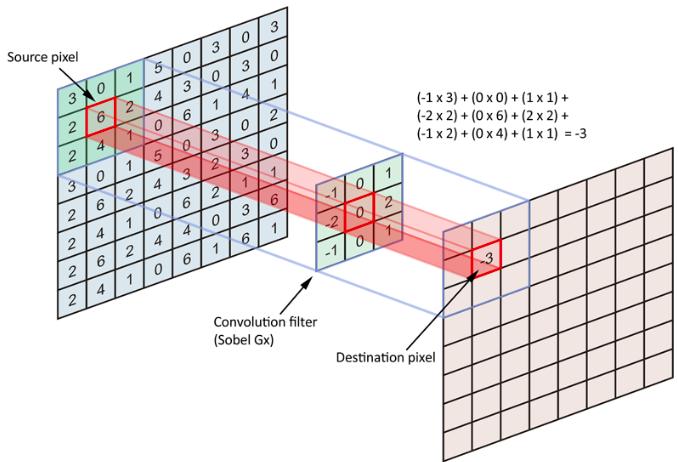
\includegraphics[width=\linewidth]{Bilder/convolutional_layer.png}
		\caption[Convolutional Layer]{Convolutional Layer \cite{DaphneCornelisse.20180424}}
		\label{convolutional_layer}
	\end{minipage}
	\hspace{.05\linewidth}% Abstand zwischen Bilder
	\begin{minipage}[b]{.4\linewidth} % [b] => Ausrichtung an \caption
		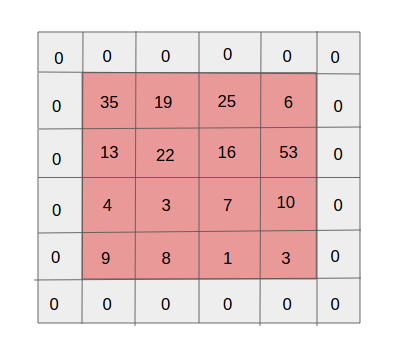
\includegraphics[width=\linewidth]{Bilder/zero_padding.png}
		\caption[Zero-Padding]{Zero-Padding \cite{AbhineetSaxena.20160629}}
		\label{zero_padding}
	\end{minipage}
\end{figure}

Ein Filter $k$ wird dazu verwendet, jeden Pixel der Eingabeschicht $I(x,y)$ nach der mathematischen Faltungsoperation 

\begin{equation}
I(x,y) = \sum_{i=1}^{n}\sum_{j=1}^{n} I(x-i, y-j)k(i,j)
\end{equation}
\equations{Mathematische Faltung}

auf die folgende Schicht abzubilden. Um keine Informationen zu verlieren und den Filter ebenso auf Randbereich anwendbar zu machen, wird oft ein sogenanntes \textit{Zero-Padding} auf eine Schicht angewandt, bei dem die Randbereiche mit LTUs des Wertes 0 aufgefüllt werden (siehe Abbildung \ref{zero_padding}) \cite{AurelienGeron.2018}.

Falls eine gleich große folgende Schicht gewünscht ist, wird eine Schrittweite (engl.: \textit{stride}) von 1 gewählt. Dies dient vor allem dazu kleinere Strukturen noch zu erkennen. Der Filter wird von einem Pixel zum direkt benachbarten Pixel bewegt und angewandt. In tieferen, fortgeschritteneren Schichten kann die Schrittweite auch größer als 1 gewählt werden, da hier bereits nach dem Anwenden mehrerer Filter feinere Muster erkannt wurden und diese nun zu größeren zusammengesetzt werden. Dabei verkleinert sich die resultierende Schicht \cite{AurelienGeron.2018}.

Das Ergebnis der Anwendung eines Filters wird als \textit{Feature Map} bezeichnet. Da mehrere Filter auf die gleiche Schicht angewandt werden, entstehen ebenso mehrere \textit{Feature Maps} der Schicht. Werden diese \textit{Feature Maps} übereinander gelagert vorgestellt, so entsteht der dreidimensionale, \glqq faltungsbedingte\grqq{} (engl.: convolutional) Charakter eines \textit{Convolutional Layers}. Eine Schicht eines \textit{Convolutional Layers} ist mit den entsprechenden Wahrnehmungsbereichen aller vorhergehenden \textit{Feature Maps} des vorhergehenden \textit{Convolutional Layers} verbunden (siehe Abbildung \ref{feature_maps}) \cite{AurelienGeron.2018}.

\begin{figure}[H]
	\begin{center}
		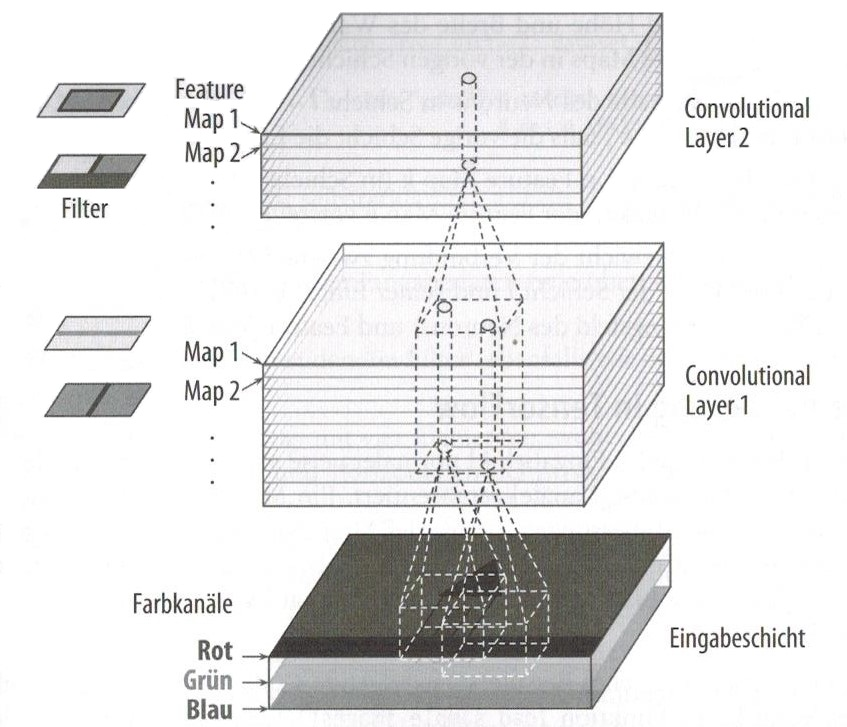
\includegraphics[width=11cm]{Bilder/feature_maps.jpeg} 
		\caption[Veranschaulichung von Feature Maps]{Veranschaulichung von Feature Maps \cite{AurelienGeron.2018}}
		\label{feature_maps}
	\end{center}
\end{figure}

Falls zusätzlich eine Farberkennung gewünscht ist, besitzt der Input Layer für jeden der drei Farbkanäle des RGB-Schemas eine Schicht, die Werte zwischen 0 und 255 in ihren LTUs tragen und den Stärken des Rot-, Grün- und Blaukanals entsprechen \cite{AurelienGeron.2018}.

Der zweite Grundbaustein eines CNN sind \textit{Pooling Layer}. Ähnlich zu den \textit{Convolutional Layern} ist auch hier jede LTU nur mit einer begrenzten Anzahl an LTUs des vorhergegangenen Layers verbunden, also nur mit dem lokalen Wahrnehmungsbereich. Der Hauptunterschied liegt aber darin, das keine Filter existieren, die die Werte vorhergehender LTUs unterschiedlich gewichten und dabei Muster erkennen. Statt den Filtern werden Aggregatfunktionen wie \textit{MAX()} oder \textit{MEAN()} dazu verwendet, um die Eingaben in nachfolgende Schichten zu verkleinern. So wird beispielsweise bei einem \textit{MAX-Pooling Layer} mit Schrittweite größer als 1 der jeweils größte Wert des lokalen Wahrnehmungsbereiches weitergereicht und damit die  Eingabe in nachfolgende Schichten verkleinert (siehe Abbildung \ref{pooling_layer}), was mit einem Informationsverlust verbunden ist. Diese Verkleinerung des Bildes ist ein wesentlicher Schritt, um bei der Mustererkennung weiter Informationen und Merkmale abstrahieren zu können \cite{AurelienGeron.2018}.

\begin{figure}[H]
	\begin{center}
		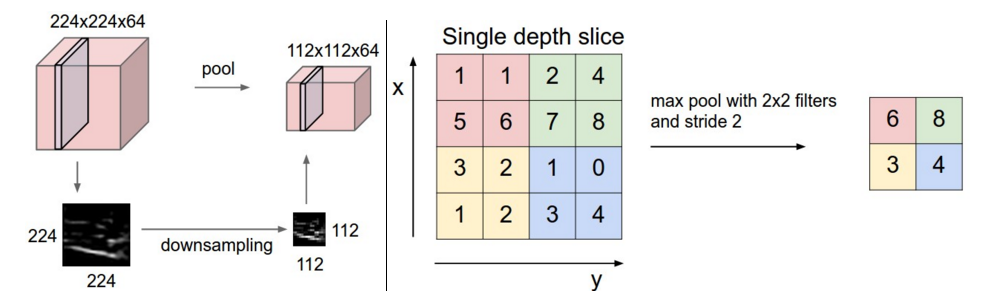
\includegraphics[width=15cm]{Bilder/pooling_layer.png} 
		\caption[Pooling Layer]{Pooling Layer \cite{LeonadroAraujoSantos.2018}}
		\label{pooling_layer}
	\end{center}
\end{figure}

Daneben ist ein Pooling über die Tiefe der \textit{Feature Maps} möglich. Hier bleibt die Größe der resultierenden \textit{Feature Maps} gleich, die Anzahl verringert sich allerdings. Die unterschiedlichen Farbkanäle werden somit nach und nach abstrahiert \cite{AurelienGeron.2018}.

Nachdem nun beide Grundbausteine eines CNNs genauer erläutert wurden, lassen sich diese nun kombinieren um ein vollständiges CNN zu bauen. Hierbei gibt es unterschiedlichste Architekturen, größtenteils äußerst komplexe. Im Rahmen dieser Arbeit genügt es allerdings, die grundlegende Architektur zu erläutern.

Diese beginnt mit einigen \textit{Convolutional Layern}, die aufeinander folgen und am Ende durch eine ReLU-Funktion nochmals gefiltert und durch ein \textit{Pooling Layer} abgeschlossen werden. Dies wird je nach Komplexität der zu erkennenden Muster und der Größe der Bilder einige Male wiederholt. Das ursprüngliche Bild wird durch die \textit{Pooling Layer} zwar immer kleiner, allerdings auch durch die \textit{Convolutional Layer} immer tiefer. Das CNN schließt mit einem normalen \textit{Feed-Forward} ANN mit \textit{Fully-Connected Layern} ab, generiert dabei einen \textit{Feature Vektor} und trifft durch eine Softmax-Funktion eine Klassifikationsaussage des Bildes \cite{AurelienGeron.2018}. 

Diese Architektur ermöglicht ebenso die Wiederverwendbarkeit einzelner Schichten und Gewichtungen für ähnliche Klassifikationsprobleme, bei denen gleiche Muster vorzufinden sind \cite{AurelienGeron.2018}.